% !TEX root = main.tex

\section{Motivation and Objectives}

\begin{itemize}
    \item CPS are increasingly everywhere
    \item many CPS are safety-critical, and a fault can literally kill people
    \item cyber threats and vulnerabilities are increasingly everywhere
    \item {\bf key assertion} traditional defense techniques are not only insufficient, they are at least in some cases unnecessary. This assertion is also true for the different paradigm of what we will call ``cyber resilience'' techniques; i.e. it is unclear whether they are necessary or sufficient
    \item {\bf another key assertion} security techniques for CPS are usually tailored for that specific application or system. There is no assurance when transitioning to other applications or techniques.
    \item therefore, we propose to understand the theory and science behind whether, when, and where different CPS security/resilience techniques are (in)effective and/or (un)necessary
\end{itemize}

\todo{bold statement about the current state of cyber and safety-critical CPS}

Consider the example in Figure~\ref{fig:motivation}, where\todo{catchy example with associated figure}

\begin{wrapfigure}{r}{0.3\linewidth}
	\centering{
		%\includegraphics[width=\linewidth,trim={142px 393px 88px 165px},clip]{figs/}
		\caption{not sure what to put here.}
		\label{fig:motivation}}	
\end{wrapfigure}

Our focus is not on improving defenses against cyber attack, or even improving detection and adaptation techniques in the face of a cyber attack. Rather, our efforts aim to\todo{understand the tradeoffs and optimize decision-making about when, where, and how to apply design patterns...}


Our approach is to develop models that can...
\begin{wrapfigure}{r}{0.6\linewidth}
	\centering{
		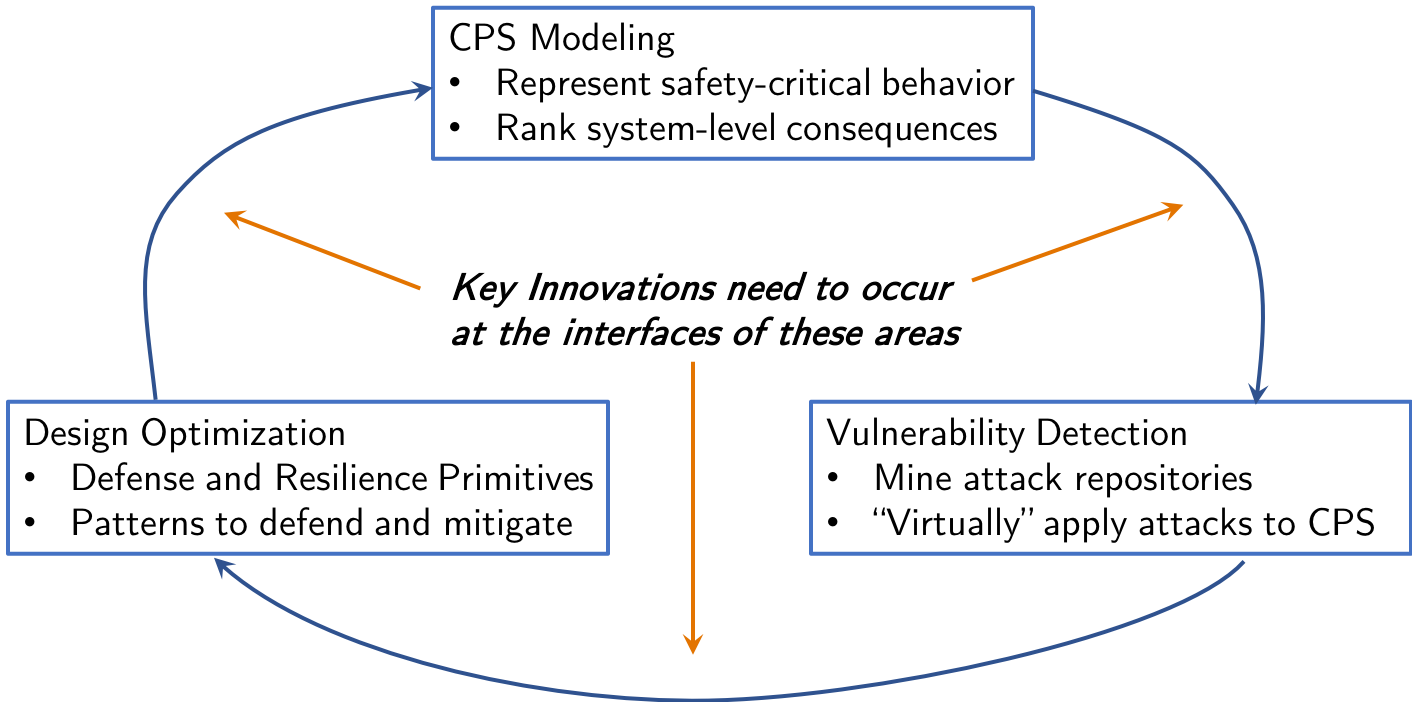
\includegraphics[width=\linewidth,trim={0 0 0 0},clip]{figs/workflow}
		\caption{Overview \hl{this is just notional, needs a good figure}}
		\label{fig:motivation}}	
\end{wrapfigure}